\chapter{A Modelagem Matemática}
\label{chap:a_modelagem_matematica}

%! Escrever um pouco sobre o que foi feito

\section{Regressão linear}
\label{sec:a_modelagem_matematica_modelo_linear}

A Regressão Linear é utilizada para analisar as relações entre o valor de uma variável resultante Y e uma ou mais variáveis X e suas interações \cite{yang2020hyperparameter}. O objetivo desta técnica é obter um modelo matemático que seja capaz de representar um fenômeno, demonstrando mediante uma relação linear as relações entre a variável de entrada e a variável de saída. Vale destacar que após a criação do modelo, é possível estimar os valores da variável de resposta Y, utilizando valores conhecidos da variável preditora X.

A Regressão Linear modela uma variável $Y$ como uma função matemática de um ou mais variáveis $X$, e então esse modelo de regressão pode ser utilizado para obter $Y$ quando apenas o $X$ é conhecido. A função matemática genérica é dada pela Equação~\ref{eq1}:

\begin{equation}\label{eq1}
    Y = \beta_1 + \beta_2 * X + \epsilon
\end{equation}
%Y = B1 + B2X + E

% Figura

Onde o $\beta_1$ é a interceptação da reta com o eixo vertical e $\beta_2$ é a inclinação ou o coeficiente angular em relação à variável, eles são chamados de coeficientes de regressão \cite{medeiros2009aplicaccao}. O parâmetro $\epsilon$ é o erro, ou seja, a porção de $Y$ que o modelo de regressão não é capaz de explicar (Figura~\ref{fig:reg-lin}).

\begin{figure}[H]
    \centering
    \caption{Representação dos coeficientes do modelo linear.}
    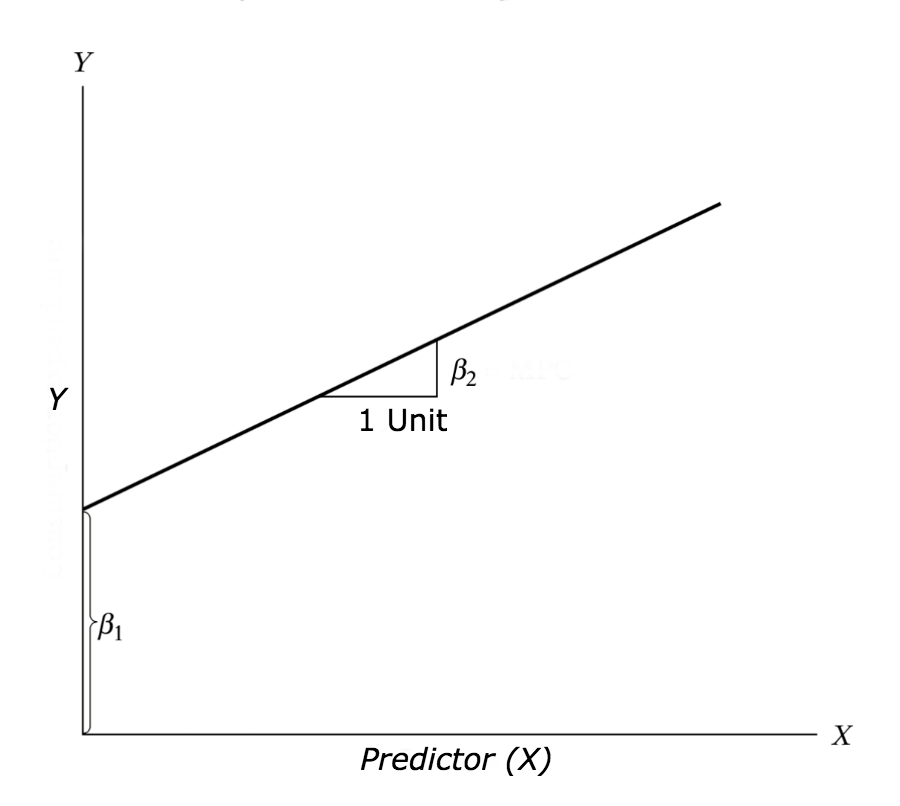
\includegraphics[width=0.8\textwidth]{images/linear-regression.png}
    \legend{Fonte: \cite{reglin}.}
    \label{fig:reg-lin}
  \end{figure}

\section{Utilizando o modelo linear de primeira ordem}
\label{sec:a_modelagem_matematica_utilizando_o_modelo_linear}

O modelo utilizado é um modelo linear múltiplo de primeira ordem, para verificar o modelo matemático utilizando o código a seguir:

%! Colocar código

\lstinputlisting[language=R, firstline=41, lastline=43,inputencoding=latin1]{code/helicoptero_teste_media.R}

Neste modelo, são utilizados todos os parâmetros (Altura, Clipe, AdesivoTopo, AdesivoLateral), de modo a verificar quais variáveis tem maior interferência sobre o modelo final e então fazer um modelo linear levando em conta estas variáveis que mais representam este modelo. Os coeficientes obtidos utilizando o modelo linear são mostrados na Tabela~\ref{tab:primor}.

% Colocar figura ou tabela
% latex table generated in R 4.0.2 by xtable 1.8-4 package
% Mon Sep 21 19:24:02 2020
\begin{table}[h]
    \centering
    \caption{Modelo linear de primeira ordem.}
    \begin{tabular}{rrrrr}
      \hline
     & Estimate & Std. Error & t value & Pr($>$$|$t$|$) \\ 
      \hline
    (Intercept) & -0.1413 & 0.0763 & -1.85 & 0.0711 \\ 
      Altura & 0.8563 & 0.0406 & 21.08 & 0.0000 \\ 
      Clipe+ & -0.1100 & 0.0325 & -3.38 & 0.0015 \\ 
      AdesivoTopo+ & 0.0592 & 0.0325 & 1.82 & 0.0757 \\ 
      AdesivoLateral+ & 0.0300 & 0.0325 & 0.92 & 0.3611 \\ 
       \hline
    \end{tabular}
    \label{tab:primor}
    \end{table}



O valor $\beta_1$, correspondente à interceptação da reta é mostrado na primeira linha. Os valores corespondentes à inclinação ($\beta_2$) são mostrados na coluna "Estimate", visto que estes são os valores correspondentes a cada variável. Logo, o modelo pode ser medido pela seguinte equação:

\begin{equation}\label{eq2}
Y = - 0.14125 + 0.85625 * Altura - 0.11 * Clipe + 0.05917 * AdesivoTopo + 0.03 * AdesivoLateral
\end{equation}

Na Equação~\ref{eq2}, a modelagem do helicóptero é dada em função da altura, da presença do clipe e dos adesivos, tanto no topo quanto na lateral. Um aspecto que também deve ser levado em consideração é o p-valor dos coeficientes do modelo linear. O p-valor indica a hipótese deve ser rejeitada ou aceita, neste caso, a hipótese é que o preditor não é significativo para o modelo. Nesta avaliação, para verificar se os preditores são significativos ou não, é verificar se os valores de $p$ são menores que 0,05.

Na análise do modelo, existem dois p-valores de dois preditores que são muito abaixo de 0.05, que são Altura e Clipe. Estes pequenos valores indicam que provavelmente Altura e Clipe sejam uma ótima adição ao modelo. Os valores de p-valor para as variáveis AdesivoTopo e Adesivo lateral são 0.076 e 0.36, respectivamente. Esses valores indicam que existe aproximadamente 8\% e 36\% de chances que essas variáveis não sejam significativas para a regressão, respectivamente.

\subsection{Residuos}

Para testar a qualidade do ajuste do modelo, um parâmetro considerado é a observação dos resíduos, que são as diferenças entre os valores reais e os valores preditos \cite{schneider2010linear}. Como a regressão linear é o processo de traçar uma reta através dos dados em um diagrama de dispersão, a reta principal representa os valores preditos. Os resíduos são a mínima distância entre os valores preditos e os valores reais, representados pelas retas vermelhas na Figura~\ref{fig:residuos}. 

% Colocar figura

\begin{figure}[H]
    \centering
    \caption{Representação dos resíduos do modelo linear.}
    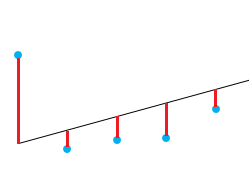
\includegraphics[width=0.5\textwidth]{images/residuos.png}
    \legend{Fonte: \cite{reglin}.}
    \label{fig:residuos}
  \end{figure}

O ideal seria que os valores de resíduos atingissem um valor igual ou próximo de zero, entretanto em aplicaçõas reais pode ser que esses valores de resíduos não sejam atingidos. No modelo testado, os valores obtidos estão situados em uma faixa entre -0.36 e 0.3, e a mádia de todos os valores atinge um valor de 0.00104, valor este muito próximo de zero.

Os gráficos gerados utilizando este modelo mostrando os residuais estão representados na Figura~\ref{fig:residuos-plot}.

\begin{figure}[H]
    \centering
    \caption{Gráficos dos resíduos do modelo linear.}
    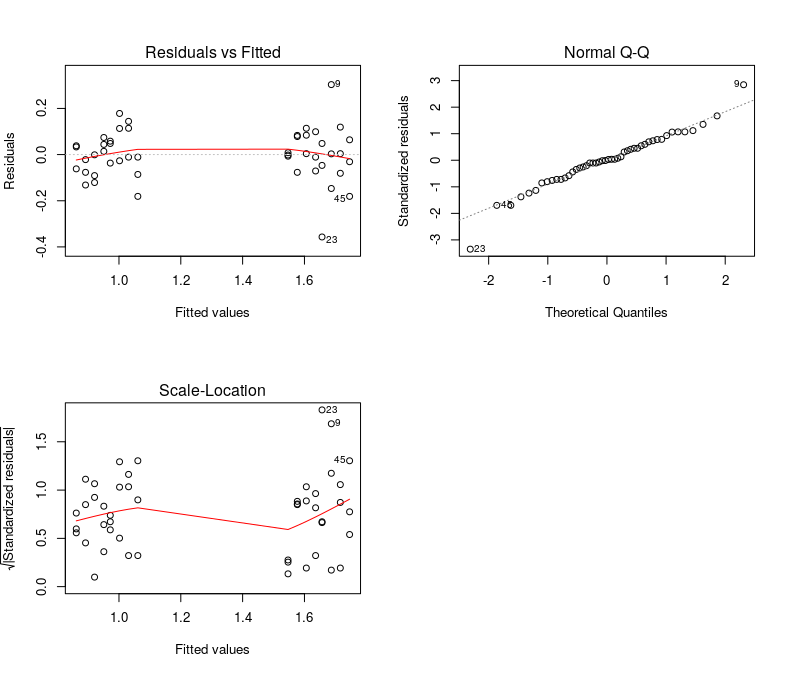
\includegraphics[width=0.8\textwidth]{images/model1ordem.png}
    \legend{Fonte: Autores.}
    \label{fig:residuos-plot}
  \end{figure}

\subsection{Múltiplo R-quadrado}

Para testar a qualidade do modelo gerado é utilizada a medida do coeficiente de determinação, ou simplesmente $R^2$, que é medido através da proporção da variabilidade total explicada pelo modelo de regressão. Para modelos que se ajustam bem aos dados, $R^2$ é próximo a 1, e modelos que se ajustam mal aos dados têm $R^2$ próximo de 0 \cite{schneider2010linear}. No modelo gerado, foi obtido um valor de $R^2$ múltiplo de 0.9145, ou seja, o modelo pode explicar 91.45\% da variabilidade total.

O modelo entrega dois valores de $R^2$ diferentes, um múltiplo e um ajustado. Uma desvantagen do $R^2$ múltiplo é que ele continuará aumentando à medida o modelo se torna mais complexo, mesmo que essas variáveis ​​não adicionem nada às previsões. O $R^2$ ajustado é uma melhor métrica caso exista mais de uma variável no modelo, uma vez que ele só cresce se erro geral das predições for reduzido. Neste caso, o valor obtido do $R^2$ ajustado é 0.9065. 


% Colocar formula







%! Escrever sobre código usado para criar o modelo linear, como este é capaz de utilizar não linearidades

\section{Utilizando o modelo linear de segunda ordem}
\label{sec:a_modelagem_matematica_o_modelo_resultante}

%! Escrever sobre o resultado encontrado e o que ele nos informa

Em seguida foi utilizado um modelo linear múltiplo de segunda ordem, para verificar se haveria alguma interação de segunda ordem significativa, além daquelas encontradas nas variáveis "Altura" e "Clipe". O modelo matemático utilizando o código a seguir:

%! Colocar código

\lstinputlisting[language=R, firstline=50, lastline=52,inputencoding=latin1]{code/helicoptero_teste_media.R}

Neste modelo, também são utilizados todos os parâmetros (Altura, Clipe, AdesivoTopo, AdesivoLateral), e as suas interações de segunda ordem. Os coeficientes obtidos utilizando o modelo linear são mostrados na Tabela~\ref{tab:segor}.

% latex table generated in R 4.0.2 by xtable 1.8-4 package
% Mon Sep 21 20:56:39 2020
\begin{table}[ht]
    \centering
    \caption{Modelo linear de segunda ordem.}
    \begin{tabular}{rrrrr}
      \hline
     & Estimate & Std. Error & t value & Pr($>$$|$t$|$) \\ 
      \hline
    (Intercept) & 0.0341 & 0.1455 & 0.23 & 0.8159 \\ 
      Altura & 0.7464 & 0.0817 & 9.14 & 0.0000 \\ 
      Clipe+ & -0.3476 & 0.1500 & -2.32 & 0.0261 \\ 
      AdesivoTopo+ & 0.0028 & 0.1500 & 0.02 & 0.9851 \\ 
      AdesivoLateral+ & -0.0039 & 0.1500 & -0.03 & 0.9796 \\ 
      Altura:Clipe+ & 0.1260 & 0.0817 & 1.54 & 0.1314 \\ 
      Altura:AdesivoTopo+ & 0.0469 & 0.0817 & 0.57 & 0.5696 \\ 
      Altura:AdesivoLateral+ & 0.0469 & 0.0817 & 0.57 & 0.5696 \\ 
      Clipe+:AdesivoTopo+ & 0.0458 & 0.0654 & 0.70 & 0.4875 \\ 
      Clipe+:AdesivoLateral+ & 0.0008 & 0.0654 & 0.01 & 0.9899 \\ 
      AdesivoTopo+:AdesivoLateral+ & -0.0925 & 0.0654 & -1.42 & 0.1654 \\ 
       \hline
    \end{tabular}
    \label{tab:segor}
    \end{table}

A modelagem do helicóptero é dada em função da altura, da presença do clipe e dos adesivos, tanto no topo quanto na lateral e ainda nas interações entre estas variáveis. Na análise do modelo, também existem dois p-valores de dois preditores que são muito abaixo de 0.05, que são $Altura$ e $Clipe$. O p-valor das variáveis $Altura$ e $Clipe$ são $5.08e^(-11)$ e $0.0261$, respectivamente. Os valores de p-valor para as demais variáveis e suas interações ultrapassam o valor de 0.05, logo, não são significativas para a regressão.

\subsection{Residuos}

No modelo testado, os valores obtidos estão situados em uma faixa entre -0.30146 e 0.29396, e a mádia de todos os valores atinge um valor de 0.01646, valor este muito próximo de zero.

Os gráficos gerados utilizando este modelo mostrando os residuais estão representados na Figura~\ref{fig:residuos-plot2}.

\begin{figure}[H]
    \centering
    \caption{Gráficos dos resíduos do modelo linear.}
    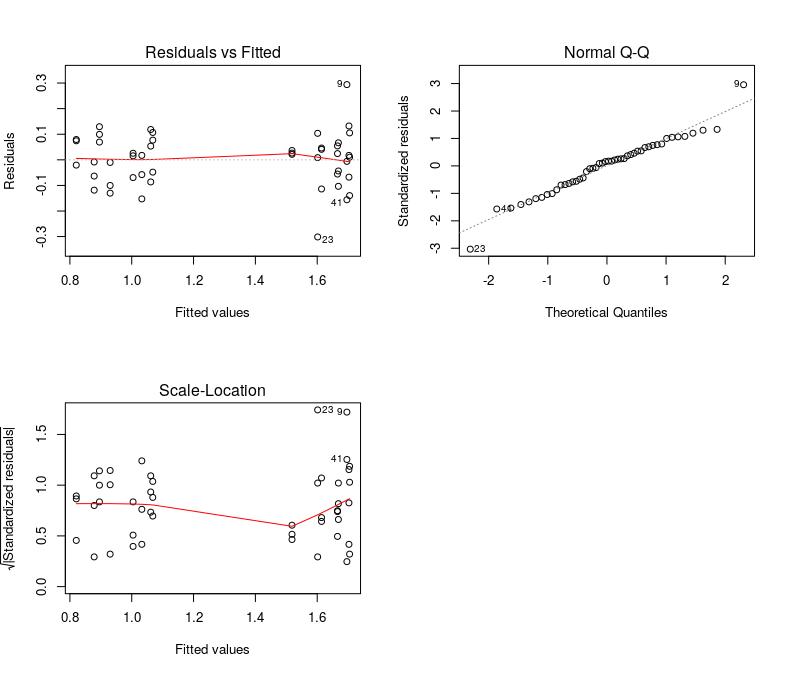
\includegraphics[width=0.8\textwidth]{images/model2ordem.png}
    \legend{Fonte: Autores.}
    \label{fig:residuos-plot2}
  \end{figure}


  \subsection{Múltiplo R-quadrado}

No modelo gerado, foi obtido um valor de $R^2$ múltiplo de 0.9256, ou seja, o modelo pode explicar 92.56\% da variabilidade total, e o valor obtido do $R^2$ ajustado é 0.9055. 

Nesta abordagem, concluiu-se que não houve uma significativa diferença entre o modelo de primeira ordem e o modelo de segunda ordem. Na comparação entre os dois modelos verificou-se que somente as variáveis "Altura" e "Clipe" eram significativas para explicar o modelo. Logo, pode-se concluir que o modelo de primeira ordem é suficiente para representar o helicóptero.